\apendice{Documentación técnica de programación}

\section{Introducción}

En este anexo se describe la documentación técnica de programación. Es decir, aquellos recursos que pretenden ser de utilidad para otros desarrolladores cuyo objetivo sea modificar el proyecto.

En primer lugar, en la sección~\ref{s:estructura-dirs}, se describirá la estructura de directorios del proyecto. A continuación, se detallará el manual del programador (sección~\ref{s:man-prog}) y se enumerarán los pasos necesarios para instalar y ejecutar el proyecto (sección~\ref{s:inst-prog}) y las herramientas auxiliares utilizadas (sección~\ref{ds:inst-aux}). Por último, se detallarán las pruebas del sistema (apartado~\ref{s:pruebas}).

\section{Estructura de directorios}
\label{s:estructura-dirs}

El repositorio del proyecto\footnote{Disponible en \url{https://github.com/phf1001/semisupervised-learning-in-cibersecurity}} inicialmente se divide en tres directorios:

\begin{itemize}
	\item \texttt{docker-deploy-kit}: incluye los \textit{scripts} necesarios para desplegar la aplicación en Docker a nivel de usuario. Su uso será detallado en la sección~\ref{s-e:docker-deploy-users}.
	\item \texttt{docs}: alberga la documentación del trabajo.
	\item \texttt{src}: contiene el código fuente de la aplicación, pruebas y recursos desarrollados, además de ficheros de configuración de herramientas y otros archivos relevanes.
\end{itemize}

Este anexo se centrará, por lo tanto, en el directorio \texttt{src}. En la ilustración~\ref{d:diag-repo-structure} se muestran las carpetas principales albergadas en este directorio. Es relevante que no todo el contenido está representado en la ilustración.

\begin{figure}[h]
	\caption[Diagrama: estructura de directorios]{Diagrama que representa la estructura física de directorios en el repositorio.}
	\centering
	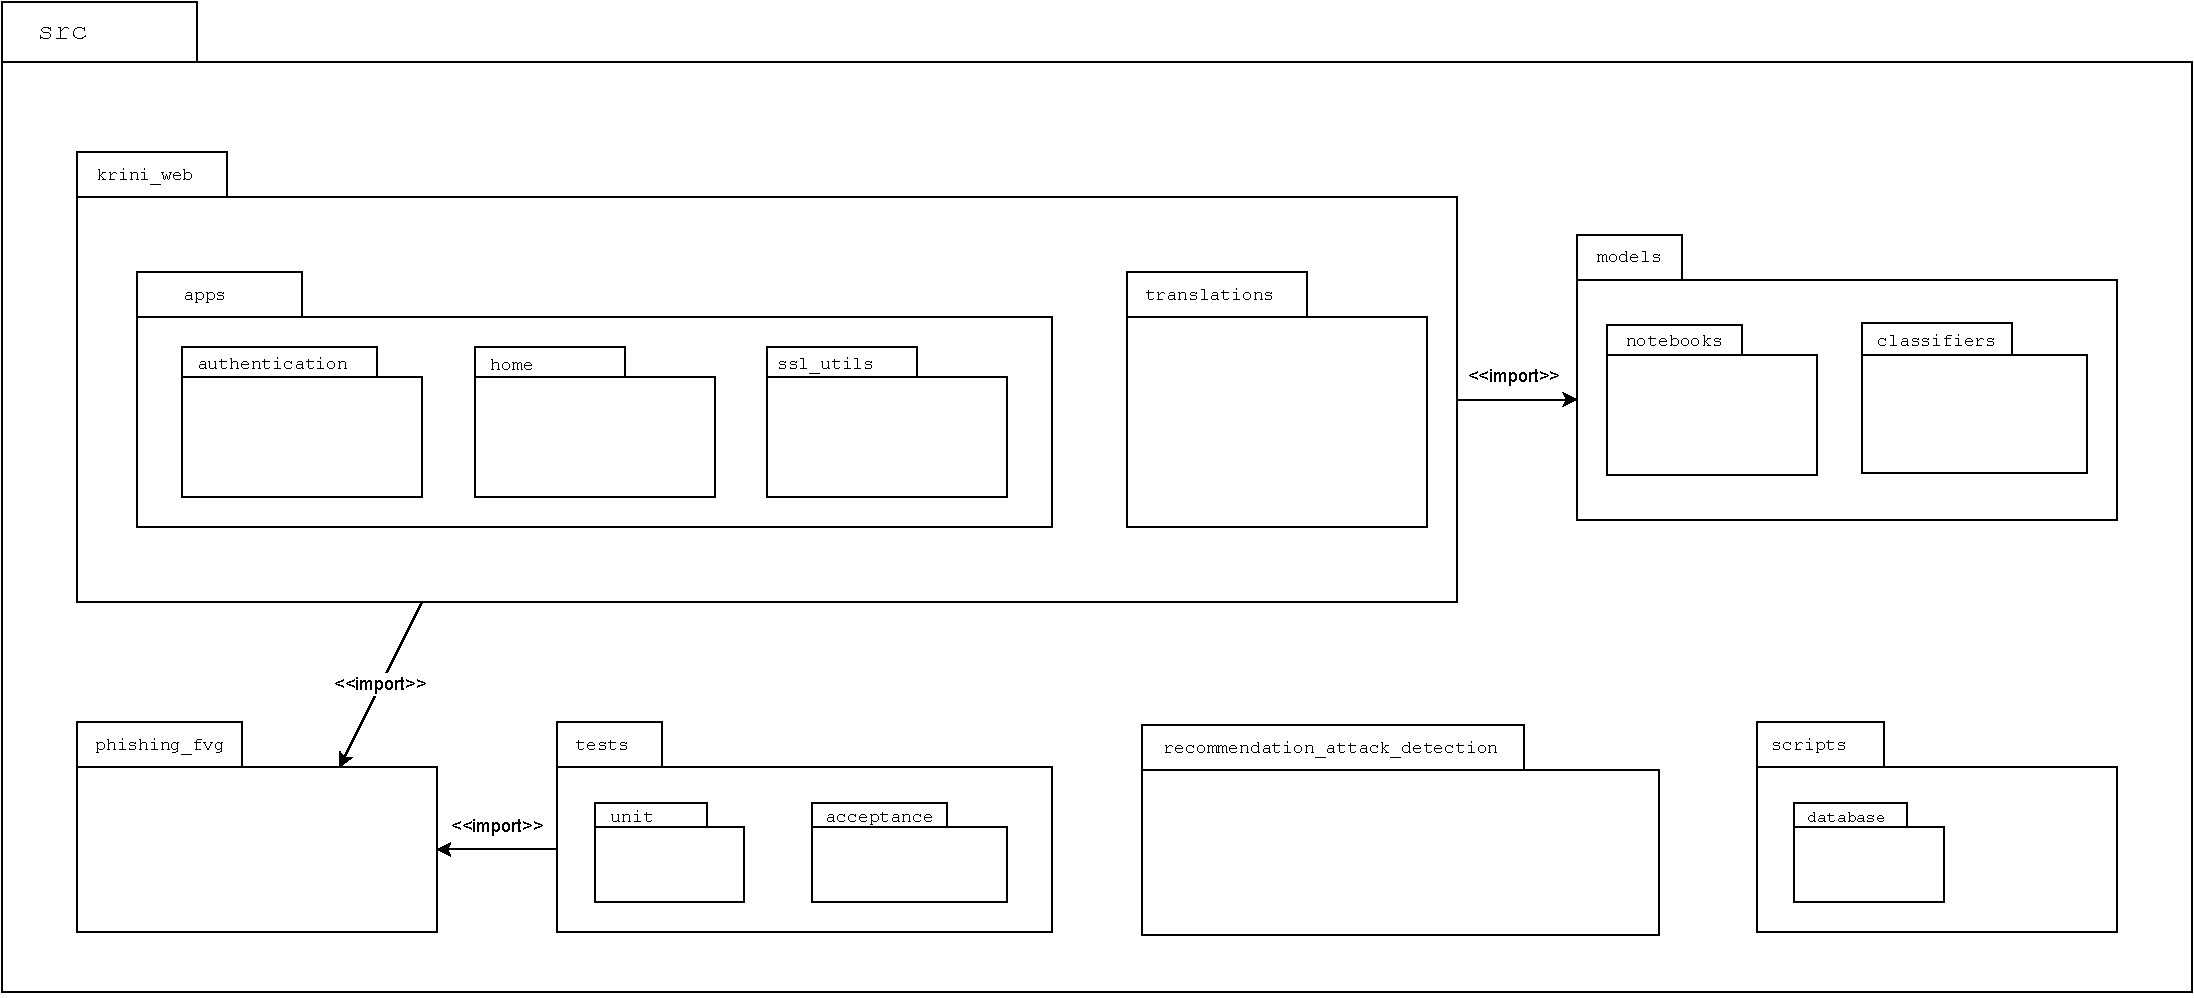
\includegraphics[width=\textwidth]{../img/anexos/diagrams/repo-structure}
	\label{d:diag-repo-structure}
\end{figure}

A continuación, se facilita una explicación más detallada del contenido de cada directorio:

\begin{itemize}
	\item \texttt{krini\_web}: alberga los recursos necesarios para la programación de la \textit{web}. 
	
	El directorio \texttt{apps} contiene la lógica de negocio principal y se divide a su vez en \texttt{authentication} (controla los inicios de sesión y registros), \texttt{home} (implementa la funcionalidad principal de la \textit{web}) y \texttt{ssl\_utils} (engloba los recursos de \textit{machine learning} necesarios así como los modelos serializados). También incluye recursos estáticos (hojas de estilos, \textit{scripts}, imágenes, etc.) en la carpeta \texttt{static} y plantillas HTML en el directorio \texttt{templates}.
	
	Hay otros directorios respectivos a entornos de programación, ficheros de configuración de servicios (Babel, Gunicorn, etc.) o \textit{scripts} de inserción de datos de prueba (\textit{mock}) para garantizar que los usuarios de Docker cuenten con recursos mínimos (carpeta \texttt{mock\_data}).
	
	\item \texttt{models}: dividido a su vez en \texttt{classifiers} y \texttt{notebooks}, alberga la implementación de los algoritmos de aprendizaje semisupervisado desarrollados y recursos auxiliares para la generación de las gráficas mostradas en la memoria.
	
	\item \texttt{phishing\_fvg}: comprende todo lo necesario para extraer vectores de características de URLs de \textit{phishing}, además de recursos necesarios (ficheros con dominios y otros datos) y resultados de experimentación. Se facilitan además \textit{notebooks} para generar gráficas o \textit{datasets}, además de un objeto TF-IDF serializado entrenado para extraer palabras clave.
	
	\item \texttt{recommendation\_attack\_detection\_fvg}: contiene los recursos necesarios para extraer vectores de características y representar los resultados de la aproximación planteada para detectar automáticamente ataques en sistemas de recomendación\footnote{El \textit{dataset} no ha sido incluído debido a su gran tamaño, pero se puede obtener en \url{https://grouplens.org/datasets/movielens/10m/}}.
	
	\item \texttt{scripts}: facilita \textit{scripts} con soluciones <<rápidas>> a problemas planteados durante el desarrollo del proyecto. Los archivos más destacables son los utilizados para levantar \textit{proxies} de Tor.

	\item \texttt{tests}: engloba las pruebas unitarias (escritas en Python y ejecutadas mediante TravisCI en cada \textit{build}) y de aceptación (programadas en Selenium).
	
	\item \textbf{Otros}: además de los directorios enumerados, también se incluyen archivos de creación de imágenes de Docker, \textit{logs}, ficheros de dependencias (\texttt{requirements.txt}), de configuración de Heroku (\texttt{runtime.txt} y \texttt{Procfile}), licencias, \texttt{README.md}, variables de producción y desarrollo, etc.
\end{itemize}



\section{Manual del programador}
\label{s:man-prog}

Habiendo descrito la estructura de directorios en la sección~\ref{s:estructura-dirs} y facilitando los detalles de instalación en las siguientes subsecciones del proyecto, son pocos los detalles que quedan por concretar en esta subsección. Por lo tanto, simplemente se pretenden facilitar ciertos detalles acerca del entorno utilizado por la desarrolladora.

\begin{itemize}

\item \textbf{Sistema Operativo}: se recomienda encarecidamente utilizar un entorno Linux para el desarrollo del proyecto. En concreto se está utilizando un Ubuntu en versión 20.4.

Como se comprobará más adelante, gran parte de los procesos requeridos se pueden desarrollar más facilmente en sistemas operativos orientados a ficheros (por ejemplo, la configuración de \textit{proxies}) o la conexión a servidores remotos.

También se ha utilizado un sistema operativo Windows para realizar pruebas de despliegue debido a que es uno de los entornos más populares.


\item \textbf{Entorno de programación}: sin pretender repetir lo expuesto en la memoria\footnote{Disponible en \url{https://github.com/phf1001/semisupervised-learning-in-cibersecurity/blob/main/docs/memoria.pdf}} (sección 4), se enumeran algunos detalles:

\begin{itemize}
	\item VSCode: como editor de código fuente.
	\item Python: en versión 3.10+ y con las dependencias mencionadas en la tabla~\ref{a:licencias}.
\end{itemize}

\item \textbf{Git y automatización del \textit{pipeline}}: actualmente, cada vez que se realiza un \textit{push} a la rama de desarrollo o la principal en Git, se lanzan ciertos procesos de control de calidad. Es importante revisar y analizar la salida proporcionada por dichas herramientas y corregir posibles defectos antes de realizar \textit{pull requests} a la rama principal.

\begin{figure}[h]
	\caption[Herramientas: control de calidad automatizado en el \textit{pipeline}.]{Herramientas de control de calidad automatizadas en el \textit{pipeline} del repositorio.}
	\centering
	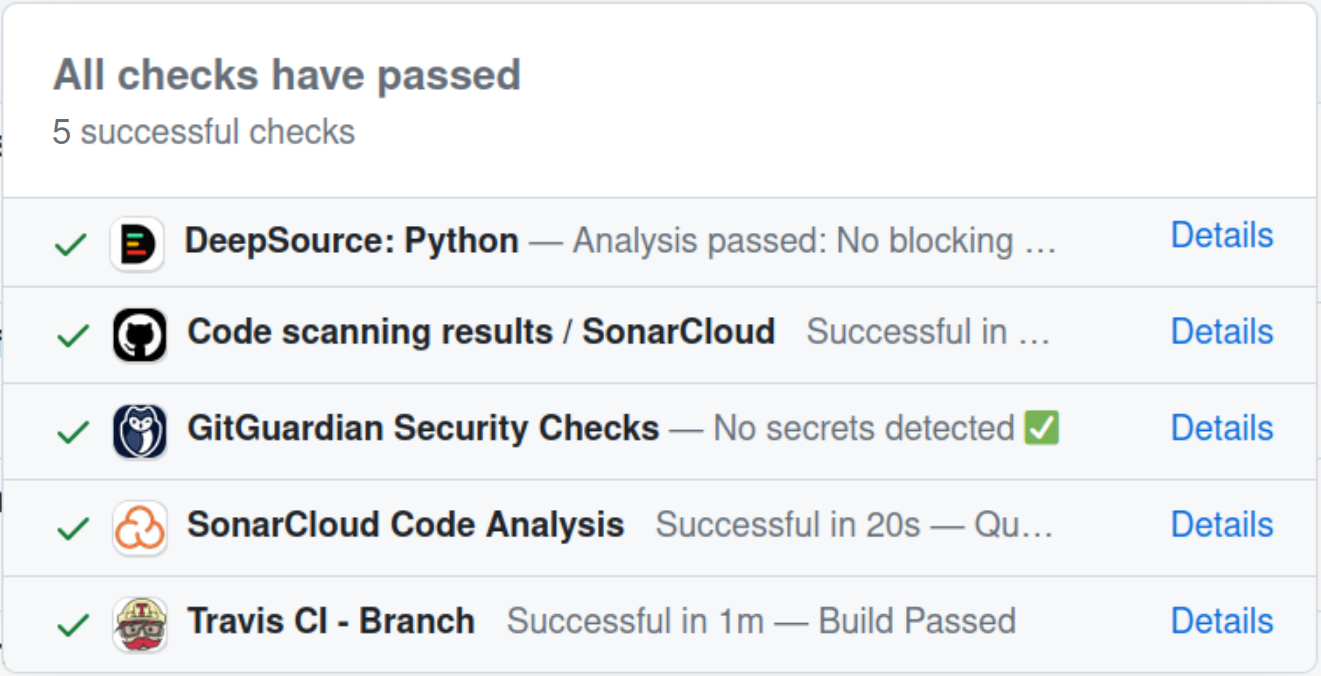
\includegraphics[scale=0.2]{../img/anexos/manual/gitpipeline}
\end{figure}

Es destacable que toda rama que se fusiona con \texttt{main} tiene que estar revisada por mínimo una persona (está protegida).

Respecto al control de ramas, se recomienda poseer una de desarrollo por cada programador. Se han realizado además otras para corregir errores o mantener registro de las \textit{release} realizadas.



\end{itemize}

\section{Compilación, instalación y ejecución del proyecto}
\label{s:inst-prog}

A continuación, se desglosan algunos de los puntos principales para poder editar el producto facilitado.

\subsection{Obtención del código fuente}

Para adquirir el código fuente de la aplicación, se puede descargar de GitHub\footnote{Disponible en \url{https://github.com/phf1001/semisupervised-learning-in-cibersecurity}} utilizando la interfaz gráfica (opción de descargar \texttt{ZIP}) o mediante un \texttt{\$ git clone}.

Para abrir el editor de código, basta con abrir una terminal en la localización del repositorio y ejecutar el comando \texttt{\$ code .}

\subsection{Entorno virtual}

Dependiendo del uso que se esté dando al repositorio (no es lo mismo simplemente ejecutar los algoritmos de apendizaje que toda la \textit{web}), se necesitan unas dependencias u otras. En función de lo requerido, se puede crear un entorno virtual u otro.

A continuación se describe cómo crear un entorno virtual genérico e instalar los requisitos necesarios para modificar y ejecutar la \textit{web}:

\begin{enumerate}
	\item Entrar en el directorio \texttt{semisupervised-learning-in-cibersecurity /src/krini\_web}
	\item Crear el entorno \texttt{\$ virtualenv env}
	\item Activar el entorno \texttt{\$ source  env/bin/activate}
	\item Instalar las dependencias \texttt{\$ pip3 install -r requirements.txt}\footnote{Por motivos de despliegue, el archivo de requerimientos se encuentra en \texttt{src} (por lo que se puede hacer previamente un \texttt{\$ cd} a la carpeta padre).}
\end{enumerate}

Cabe destacar que para desplegar en herramientas que necesitan menos recursos (por ejemplo, TravisCI, que ejecuta pruebas unitarias) se han creado ficheros de requerimientos personalizados que se encuentran en sus respectivas carpetas.


\subsection{Generación de \textit{datasets} para \textit{phishing}}

Cuando se quieran generar vectores de características para un número elevado de instancias, se recomienda hacerlo protegiendo la identidad del usuario mediante el uso de un \textit{proxy} de Tor. Para ello:

\begin{enumerate}
	\item Entrar en el directorio \texttt{semisupervised-learning-in-cibersecurity /src/scripts}
	\item Lanzar el \textit{script} para levantar \textit{proxies} mediante el comando \texttt{\$ sudo python3 proxies\_launcher.py}
	\item Introducir por teclado el número de \textit{proxies} deseados y esperar a que se levanten.
	\item Generar el \textit{dataset} ejecutando el \textit{notebook} \texttt{phishing\_dataset\_generator .ipynb} mediante VSCode.
\end{enumerate}

\subsection{Ejecución de experimentos en remoto}

Hay ocasiones en las que los experimentos lanzados requieren una cantidad muy elevada de recursos. En dichos casos, lo mejor es ejecutar los \textit{scripts} en servidores de mayor envergadura. Para ello se seguirán los siguientes pasos:

\begin{enumerate}
	\item Activar la \texttt{vpn} de la UBU\footnote{\url{https://www.ubu.es/servicio-de-informatica-y-comunicaciones/documentacion-de-ayuda/manuales-de-usuario/manuales-vpn}} (se requiere autorización previa).
	\item Acceder al servidor deseado vía \texttt{ssh}. Para ello, ejecutar el comando \texttt{ssh -X -p 22 usuario@ipmáquina} y autenticarse.
	\item Si es la primera ejecución:
		\begin{enumerate}
			\item Descargar el repositorio deseado mediante \texttt{git} o copiar los archivos mediante el comando \texttt{\$ scp -r ubicaciónlocal usuario} \texttt{@ipmáquina:ubicaciónremota}. Si se usa el comando \texttt{\$ scp}, hacerlo desde local.
			\item Crear un entorno virtual (o copiar uno existente mediante \texttt{scp} en caso de falta de permisos).
		\end{enumerate}
	\item Para evitar que el proceso lanzado se muera al cerrar el \texttt{ssh}, abrir una terminal de \texttt{tmux} mediante el comando \texttt{\$ tmux}.
	\item Activar el entorno virtual.
	\item Lanzar el \textit{script} deseado desde \texttt{tmux} mediante el comando \texttt{python3 script.py}.
	\item Desacoplar la terminal pulsando \texttt{Ctrl + b y luego d}.
	\item Comprobar que el \textit{script} se está ejecutando mediante \texttt{ps -fA | grep python}
	\item Consultar los \textit{logs} mediante el comando \texttt{\$ nano} o \texttt{\$ tail}.
	\item Copiar los ficheros resultantes a local mediante \texttt{\$ scp}.
	\item Si se quiere recuperar la terminal desacoplada, hacerlo mediante \texttt{\$ tmux attach}.
\end{enumerate}

\subsection{\textit{Web}: Despliegue en local (Flask y PostgreSQL)}
\label{s-d:flask-deploy}
Para programar y probar la aplicación \textit{web}, se recomienda utilizar el propio servidor de Flask. Para ello, se han de seguir los siguientes pasos:

\begin{enumerate}
	\item Entrar en el directorio \texttt{\$ semisupervised-learning-in-cibersecurity /src/krini\_web}
	\item Activar el entorno virtual \texttt{\$ . env/bin/activate}
	\item Asegurarse de que el fichero \texttt{run.py} tiene el modo \texttt{DEBUG} en \texttt{default = True}.
	\item Exportar las variables de entorno \texttt{\$ export FLASK\_APP=run.py}
	\item Activar el modo depuración \texttt{\$ export FLASK\_ENV=development}
	\item Lanzar el servidor mediante el comando \texttt{\$ flask run --host=127.0.0.1 --port=5000}. Evidentemente, se pueden configurar las direcciones y puertos que se considere necesario.
\end{enumerate}

Algunas anotaciones al respecto:

\begin{itemize}
	\item Para desarrollo, se ha utilizado una base de datos PostgreSQL en \texttt{localhost}. En Ubuntu se puede configurar siguiendo las instrucciones mostradas en~\cite{postgrelocal}. Es importante contar con una base de datos llamada \texttt{krini}, un usuario \texttt{dev} con privilegios y contraseña \texttt{123}. Las tablas se crean solas (mediante SQLAlchemy) al visitar la aplicación.
	\item La conexión con la base de datos se ha gestionado principalmente mediante línea de comandos. Para ello, basta con vincularse mediante \texttt{\$ psql -U dev -h 127.0.0.1 -d krini} y utilizar la sintáxis de SQL.
	\item La \textit{web} está basada en una plantilla para aplicaciones Flask llamada Argon Dashboard\footnote{\url{https://github.com/creativetimofficial/argon-dashboard}}.
\end{itemize}

\subsubsection{Compilar y modificar los archivos de idiomas}

Cuando se introduzca una cadena nueva en el programa, se debe etiquetar mediante la función \texttt{gettext()} o \texttt{lazy\_gettext()} (en función del tipo de traducción deseada). Posteriormente, se han de seguir los pasos mostrados a continuación~\cite{pybabelmanual}:

\begin{enumerate}
	\item Entrar en el directorio \texttt{\$ semisupervised-learning-in-cibersecurity /src/krini\_web}
	\item Activar el entorno virtual \texttt{\$ . env/bin/activate}
	\item Actualizar el fichero \texttt{.pot \$ pybabel extract -F babel.cfg -o}
	
	\texttt{ messages.pot --input-dirs=. }
	\item La primera vez, generar los ficheros \texttt{.po} y \texttt{.mo} mediante el comando \texttt{\$pybabel init -i messages.pot -d translations -l <idioma>} .
	Las veces sucesivas, simplemente actualizar mediante el comando \texttt{\$pybabel update -i messages.pot -d}.
	\item Realizar los cambios que se desee en el fichero \texttt{.po}.
	\item Compilar las modificaciones \texttt{\$ pybabel compile -d translations}. 
\end{enumerate}

\subsection{\textit{Web}: Actualización de imágenes de Docker}

Para garantizar que la aplicación pueda ejecutarse independientemente del sistema anfitrión, se han utilizado contenedores de Docker.

A nivel de usuario se ha automatizado el despliegue mediante \textit{scripts} multiplataforma\footnote{Disponibles en \url{https://github.com/phf1001/semisupervised-learning-in-cibersecurity/tree/main/docker-deploy-kit}} que descargan las imágenes del repositorio de DockerHub\footnote{Disponible en \url{https://hub.docker.com/r/phf1001/krini}} de la autora~\cite{dockerHub}. Los pasos necesarios serán descritos en la correspondiente sección del manual de usuario~\ref{s-e:docker-deploy-users}.

A nivel de programador, se ha configurado el archivo \texttt{DockerFile} que genera una imagen de Python en la que se copia la carpeta \texttt{src} del repositorio e instala el archivo \texttt{requirements.txt}. Para levantar los contenedores, se facilita el correspondiente archivo \texttt{docker-compose}, que lanza la \textit{web} y una base de datos PostgreSQL~\cite{dockerFlaskPostgre}. Para hacer la base de datos persistente y evitar que se reinicie cada vez que se levanta la imagen, se ha mapeado un volumen \texttt{data}~\cite{dockerPersist}.

Además, para que los usuarios no tengan la base de datos vacía, se ha creado un \textit{script} de Python (\texttt{krini\_web/mock\_data/fill\_database.py}) que se ejecuta en el contenedor gracias al \texttt{docker-compose} e inserta usuarios, modelos, URLs y reportes. Está copiado en la imagen.

De esta forma, cuando un programador quiera actualizar las imágenes de Docker debe:

\begin{enumerate}
	\item Entrar en el directorio raíz del repositorio \texttt{\$ semisupervised-learning -in-cibersecurity}.
	\item Ejecutar el comando \texttt{\$ docker-compose build --no-cache}.
	\item Ejecutar el comando \texttt{\$ docker-compose -f docker-compose.yml} \texttt{up -d --build}.
	\item Comprobar que ambas imágenes están disponibles mediante \texttt{\$ docker images -a}.
	\item Actualizar la web en DockerHub mediante \texttt{\$ docker tag semisupervi sed -learning-in-cibersecurity\_web phf1001/krini:web-<n> \&\& docker push phf1001/krini:web-v<n>}
	\item Actualizar la base de datos en DockerHub mediante \texttt{\$ docker tag postgres phf1001/krini:db-v<n> \&\& docker push phf1001/krini :db-v<n>}
	\item Cambiar las versiones en los \texttt{docker-compose} para los clientes.
\end{enumerate}

Algunos comentarios al respecto:

\begin{itemize}
	\item Durante el desarrollo, a veces se ha dejado el puerto 5432 expuesto por motivos de comodidad (acceso a la base de datos por terminal). Si Docker avisa de que no puede levantar contenedores ya que el puerto esta ocupado, se recomienda ejecutar \texttt{\$ sudo netstat -p -nlp | grep 5432} para comprobar por quién y, si se está de acuerdo, matar el proceso mediante \texttt{sudo kill <PID>}. Si no se necesitan los puertos, también se puede eliminar el campo \texttt{ports} del \texttt{docker-compose}
	
	\item Se dispone de un \textit{script} tanto en \texttt{.sh} como en \texttt{.bat} llamado \texttt{docker-clean} que pausa, limpia y elimina contenedores (e imágenes) para liberar recursos. 
\end{itemize}


\subsection{\textit{Web}: Despliegue en Heroku}

El despliegue en Heroku se complica un poco más de lo habitual por la estructura de directorios creada (la aplicación \textit{web} se encuentra varias carpetas alejada de la raíz y hace uso de elementos externos).

Los pasos seguidos para desplegar la aplicación se pueden consultar en~\cite{herokudeploy}. Es destacable la necesidad de crear un archivo \texttt{Procfile} (define los pasos que se ejecutan al iniciar la aplicación~\cite{herokuprocfile}) que se encuentre en la raíz del directorio que se quiere desplegar (en este caso, sólo \texttt{src}, no tiene sentido subir la documentación) junto con el archivo \texttt{requirements.txt} de la \textit{web}. Además, se ha incluído un fichero \texttt{runtime.txt} para indicar la versión de Python deseada.

Nótese que el fichero \texttt{Procfile} ejecuta \texttt{\$ web: cd krini \_web \&\& guni corn run:app --preload --workers 4 --timeout 0 --log-file=-} (por la necesidad comentada de cambiar de directorio ya que se encuentra dentro de \texttt{src} para que Heroku encuentre la aplicación). Al igual que en Docker, se ha utilizado un servidor Gunicorn por ser un servidor WSGI\footnote{\textit{Web Server Gateway Interface}: especificación que describe cómo se comunica un servidor \textit{web} con una aplicación \textit{web} y cómo se procesan las solicitudes/peticiones.} compatible con varios \textit{frameworks} (entre ellos, Flask).

Para desplegar únicamente \texttt{src}~\cite{herokusubtree}, el comando clásico se complica un poco. Los pasos son:

\begin{enumerate}
	\item Entrar en el directorio raíz del repositorio \texttt{\$ semisupervised-learning -in-cibersecurity}.
	\item Ejecutar el comando \texttt{\$ git subtree push --prefix src/ heroku main
	}. Es probable que requiera un inicio de sesión.
\end{enumerate}

Algunos detalles a tener en cuenta:

\begin{itemize}
	\item La base de datos PostgreSQL de la \textit{web} también se ha desplegado en Heroku mediante un \textit{add-on} y es accesible por CLI mediante el comando \texttt{\$heroku pg:psql <base> --app krini}. En código, se recupera la URI de conexión mediante variables de entorno.
	\item Es importante destacar que, para que la \textit{web} desplegada pueda utilizar \texttt{https}, es necesario activar los certificados SSL\footnote{Un certificado SSL (\textit{secure socket layer}) permite cifrar la conexión entre cliente y servidor, además de autentificar una \textit{web} como legítima.} y renovarlos cada tres meses. El proceso acerca de cómo hacerlo se puede consultar en la documentación oficial de Heroku\footnote{Disponible en: \url{https://devcenter.heroku.com/articles/ssl}}.
\end{itemize}


\section{Compilación, instalación y ejecución de herramientas auxiliares}
\label{ds:inst-aux}

Se enumeran a continuación algunas herramientas auxiliares utilizadas durante el desarrollo del proyecto y se facilitan los pasos para ejecutar su despliegue.
\begin{figure}[h]
	\caption[Herramientas auxiliares: experimento en KEEL]{Configuración de un experimento que utiliza el algoritmo \textit{co-forest} mediante la GUI de KEEL.}
	\centering
	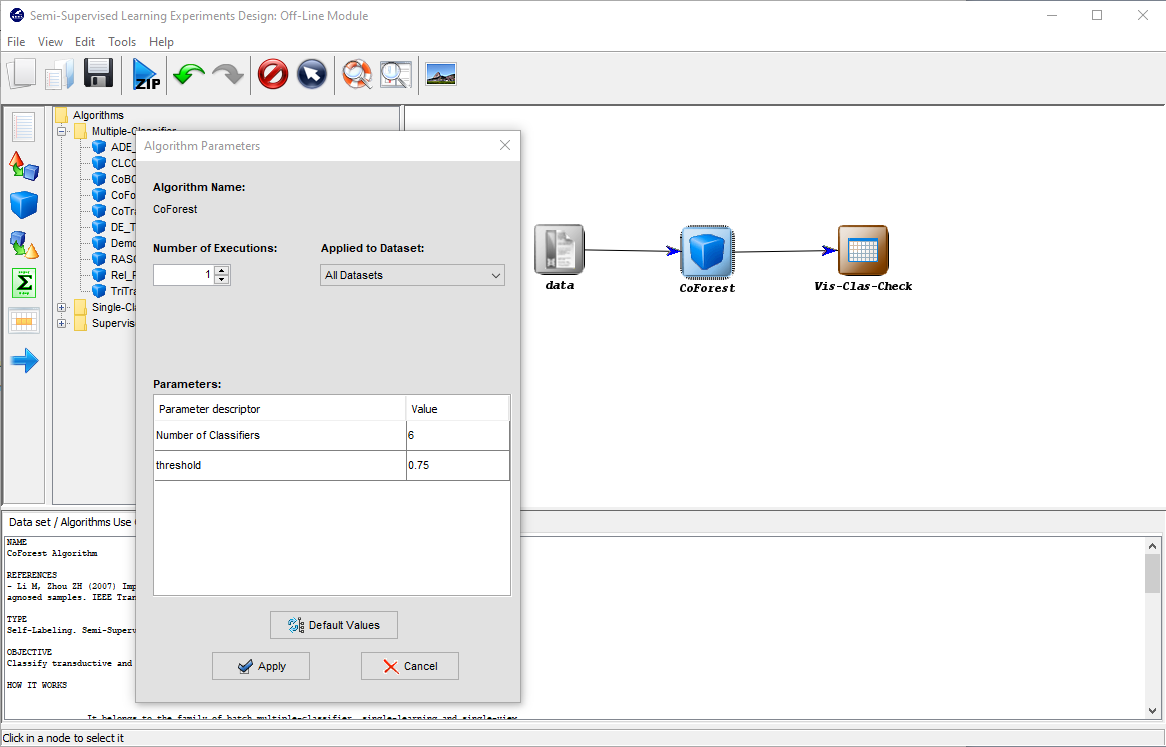
\includegraphics[scale=0.5]{../img/anexos/manual/keel_gui.png}
\end{figure}

\subsection{KEEL}

KEEL es una herramienta que permite experimentar con modelos de \textit{machine learning}. Ha sido creada por distintas universidades españolas y financiada por el Ministerio de Educación y Ciencia~\cite{KEEL}.

Para poder ejecutarla, en primer lugar, se han de descargar los ficheros fuente del repositorio de GitHub~\cite{keelRepo}. Una vez se han descargado, se compilan aprovechando el fichero \texttt{build.xmlz} contenido y la herramienta \texttt{ant}. Mediante el comando \texttt{ant cleanAll} se eliminan recursos previos (para evitar conflictos), y mediante el comando \texttt{ant} se compila el código fuente.

Posteriormente se ejecuta la aplicación mediante el comando \texttt{java -jar ./dist/GraphInterKeel.jar} y se utiliza mediante su interfaz gráfica.


\section{Pruebas del sistema}
\label{s:pruebas}

Las pruebas \textit{software} son un proceso sistemático y controlado para evaluar y verificar el correcto funcionamiento de un producto. Están reguladas por la ISO/IEC/IEEE 29119~\cite{iso-pruebas} y son fundamentales ya que permiten detectar errores y defectos antes del despliegue, pudiendo así ahorrar costos, tiempo, y facilitando la satisfacción del cliente.

Existen distintos tipos de pruebas en función de qué se está evaluando. Generalmente se sigue un enfoque de más bajo nivel a más alto nivel, iniciando en las pruebas unitarias y finalizando en las pruebas de aceptación.


\subsection{Pruebas unitarias}
\label{s:pruebas-unitarias}

Las pruebas unitarias se centran en comprobar el correcto funcionamiento de las partes individuales del \textit{software}. Se llevan a cabo a nivel de código y están diseñadas para detectar errores y defectos en unidades de menor tamaño (por ejemplo funciones o clases).

Debido a que los algoritmos de ML cuentan con pruebas independientes (comparaciones con otras implementaciones) y la \textit{web} cuenta con las pruebas descritas en la sección~\ref{s:pruebas-aceptación}, se han realizado pruebas unitarias para la clase de utilidades \texttt{phishing\_utils}.

Además, las pruebas unitarias se han automatizado mediante Travis CI, de forma que cada vez que se hace un \textit{push} a las ramas principales o de desarrollo se dispara una \textit{build} que las ejecuta automáticamente como se muestra en la imagen~\ref{d:cp-travis}.

\begin{figure}[h]
	\caption[TravisCI: ejecución automática de pruebas unitarias]{Ejecución automática de las pruebas unitarias mediante TravisCI.}
	\centering
	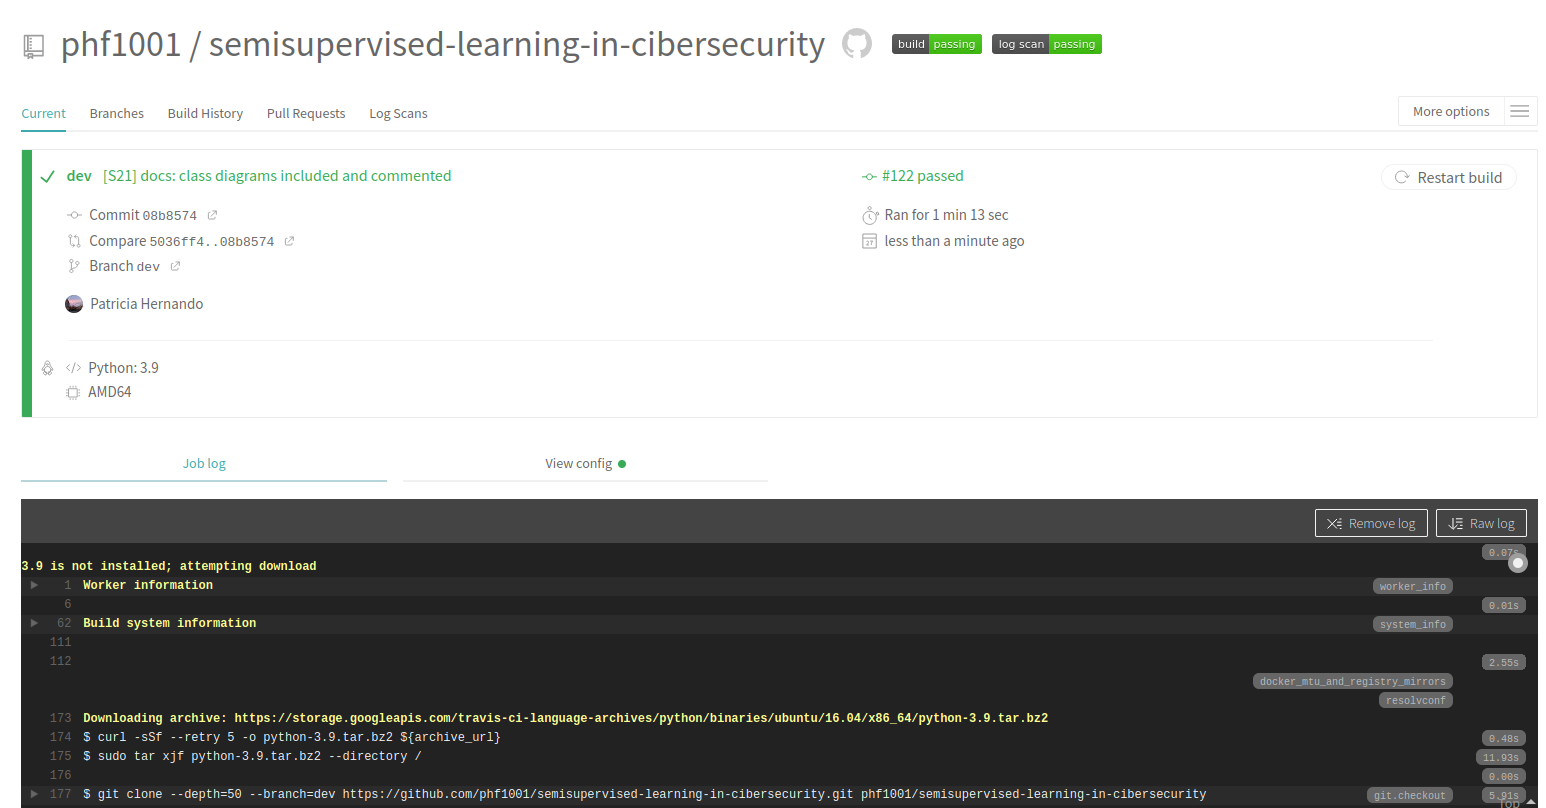
\includegraphics[width=\textwidth]{../img/anexos/cp/travis-tests}
	\label{d:cp-travis}
\end{figure}


\subsection{Pruebas de aceptación}
\label{s:pruebas-aceptación}

Las pruebas de aceptación se realizan para verificar si el \textit{software} está listo para su implementación y si cumple con los criterios de aceptación del cliente. En este proyecto se han querido evaluar algunos de los casos más <<extraños>> con el fin de comprobar su correcto funcionamiento. Estos se han organizado en tres \textit{test suites} divididas por categorías.

Todos los casos de prueba mostrados en las tablas han sido automatizados utilizando Selenium (como se puede observar en la imagen~\ref{cp:selenium}). Los \textit{test} se facilitan en el repositorio de la aplicación, además de los datos necesarios para ejecutarlos.

\begin{figure}[h]
	\caption[Selenium: ejecución automática de pruebas de aceptación]{Ejecución automática de las pruebas de aceptación y seguridad con la herramienta Selenium.}
	\centering
	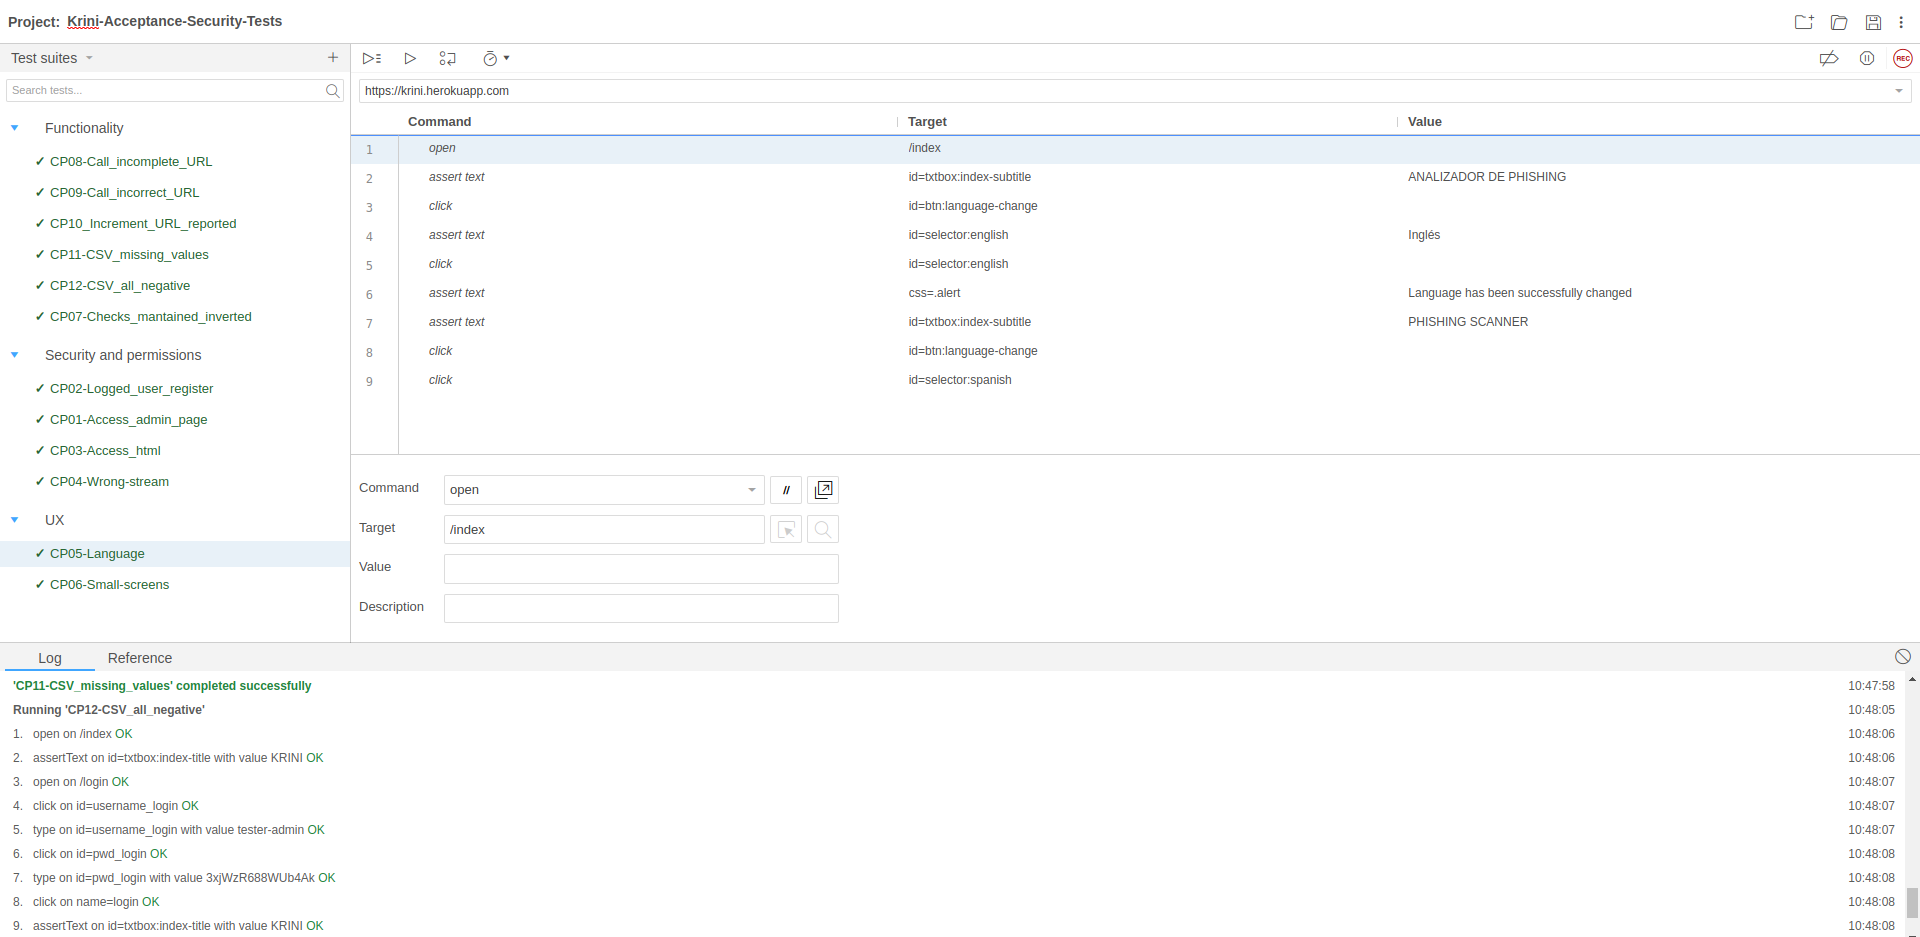
\includegraphics[width=\textwidth]{../img/anexos/cp/selenium-tests}
	\label{cp:selenium}
\end{figure}

\begin{table}[p]
	\centering
	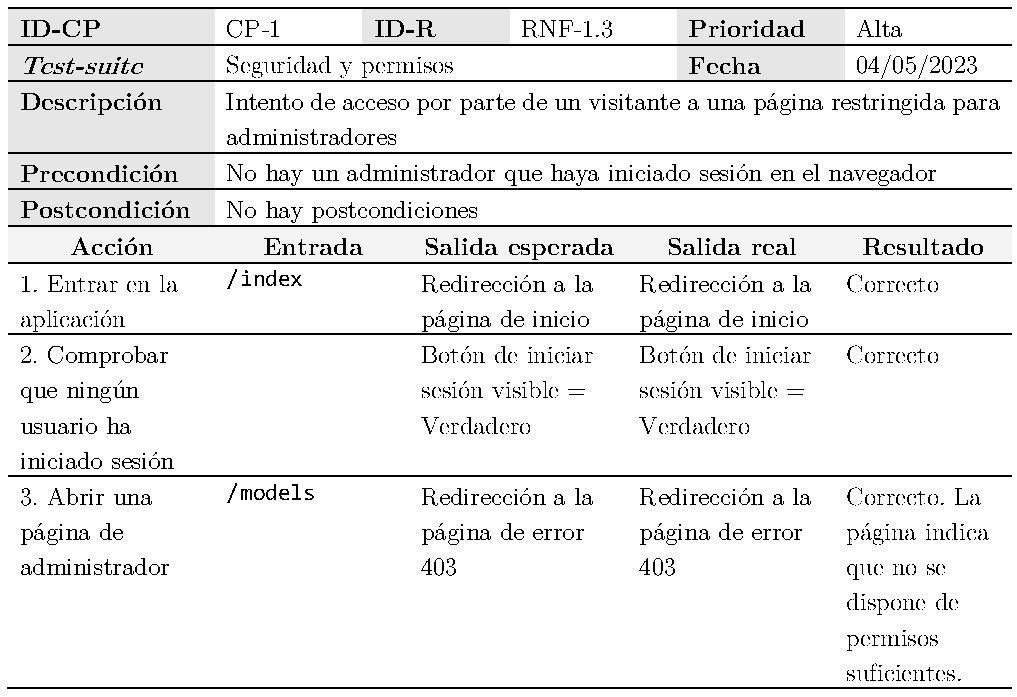
\includegraphics[width=\textwidth]{../img/anexos/cp/CP-1}
	\caption{CP-1 Acceso a página restringida.}
	\label{cp:acc-restringido}
\end{table}

\begin{table}[p]
	\centering
	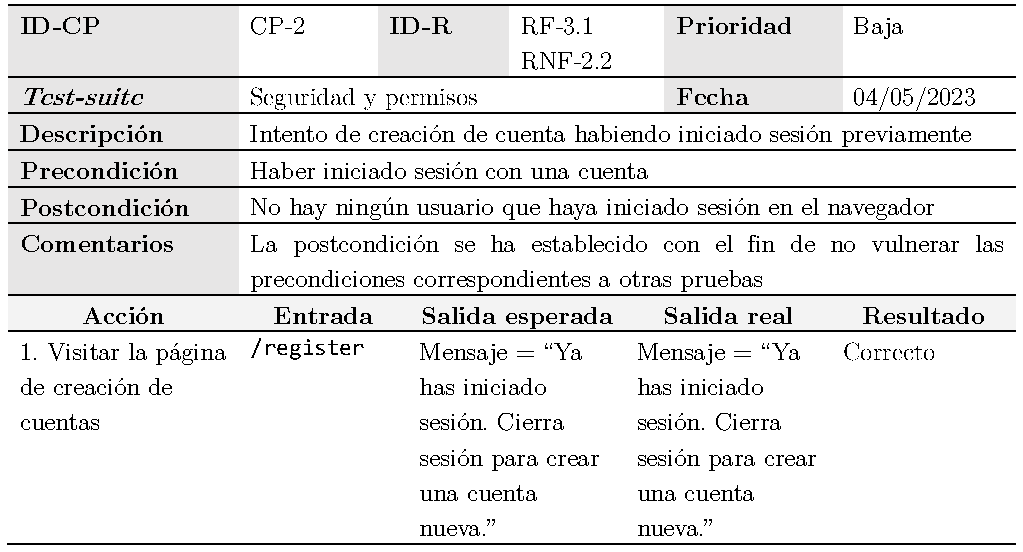
\includegraphics[width=\textwidth]{../img/anexos/cp/CP-2}
	\caption{CP-2 Intento de registro con cuenta accedida.}
	\label{cp:registro}
\end{table}

\begin{table}[p]
	\centering
	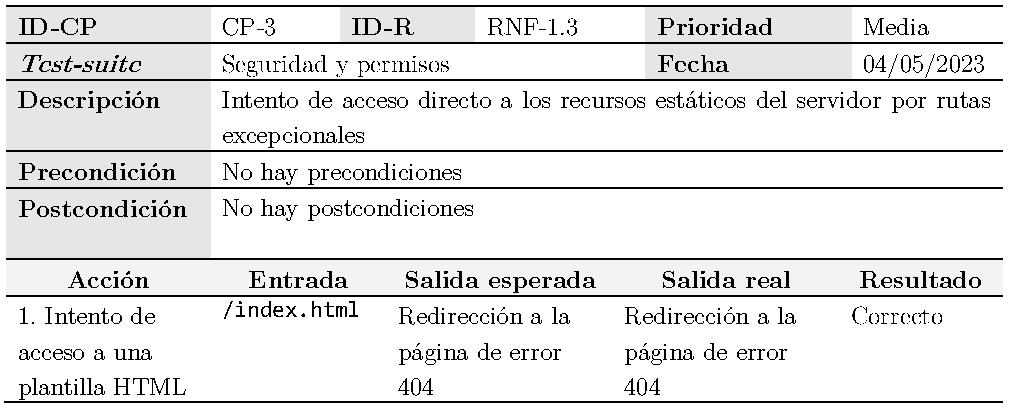
\includegraphics[width=\textwidth]{../img/anexos/cp/CP-3}
	\caption{CP-3 Acceso a recursos estáticos.}
	\label{cp:acc-html}
\end{table}

\begin{table}[p]
	\centering
	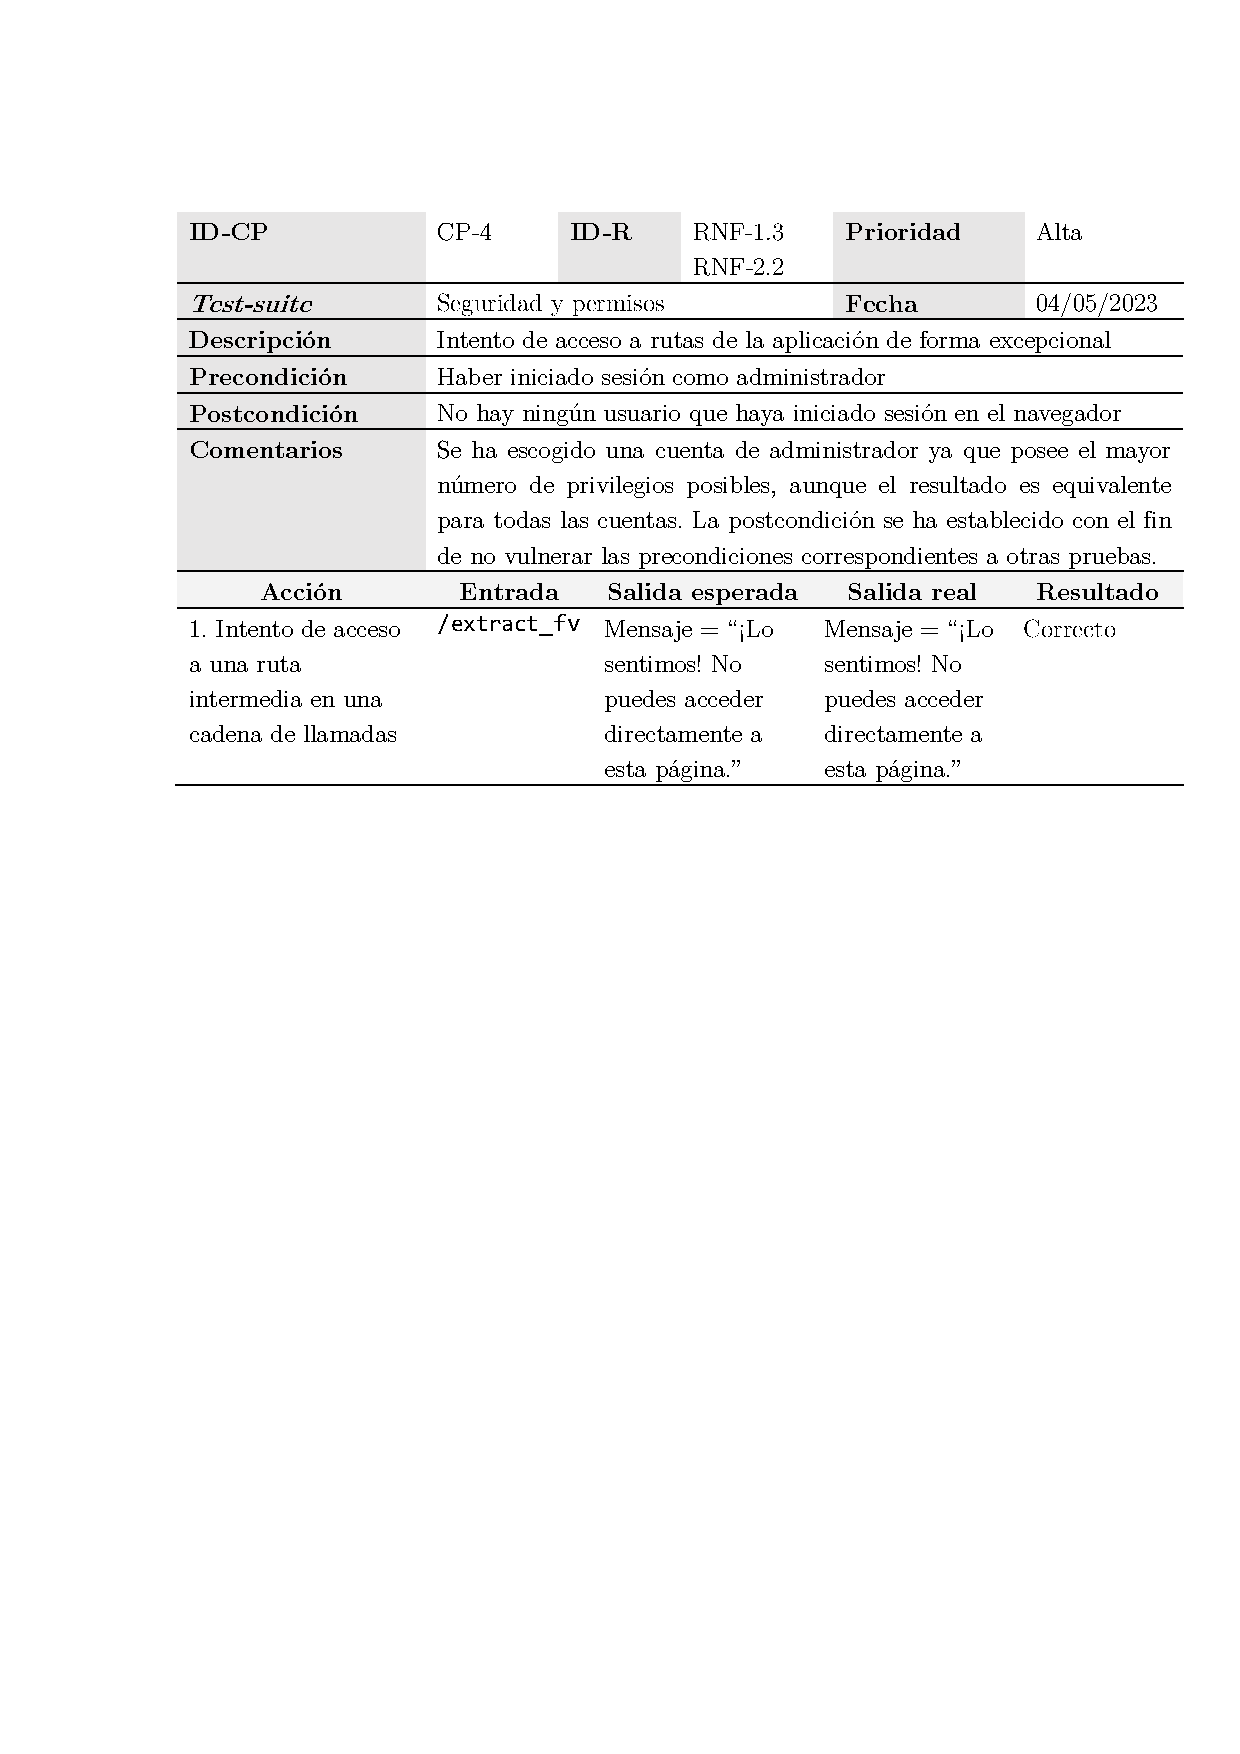
\includegraphics[width=\textwidth]{../img/anexos/cp/CP-4}
	\caption{CP-4 Acceso a rutas excepcionales.}
	\label{cp:wrong-stream}
\end{table}

\begin{table}[p]
	\centering
	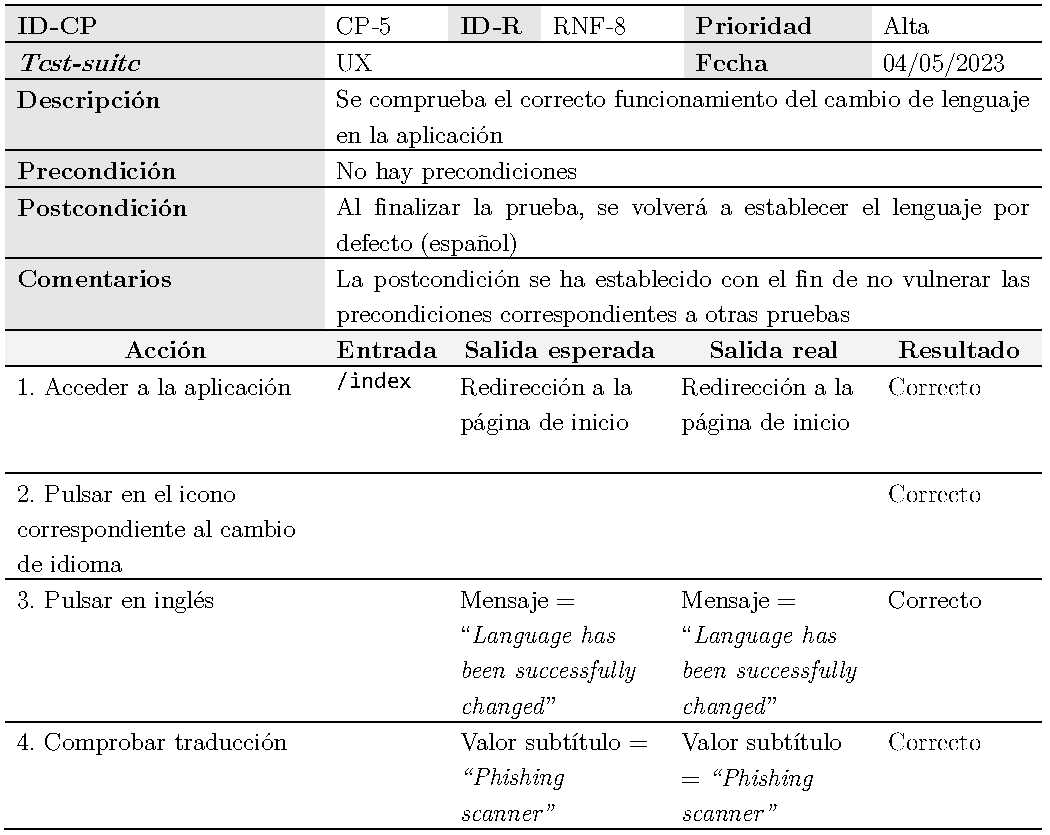
\includegraphics[width=\textwidth]{../img/anexos/cp/CP-5}
	\caption{CP-5 Cambio de idioma.}
	\label{cp:language}
\end{table}

\begin{table}[p]
	\centering
	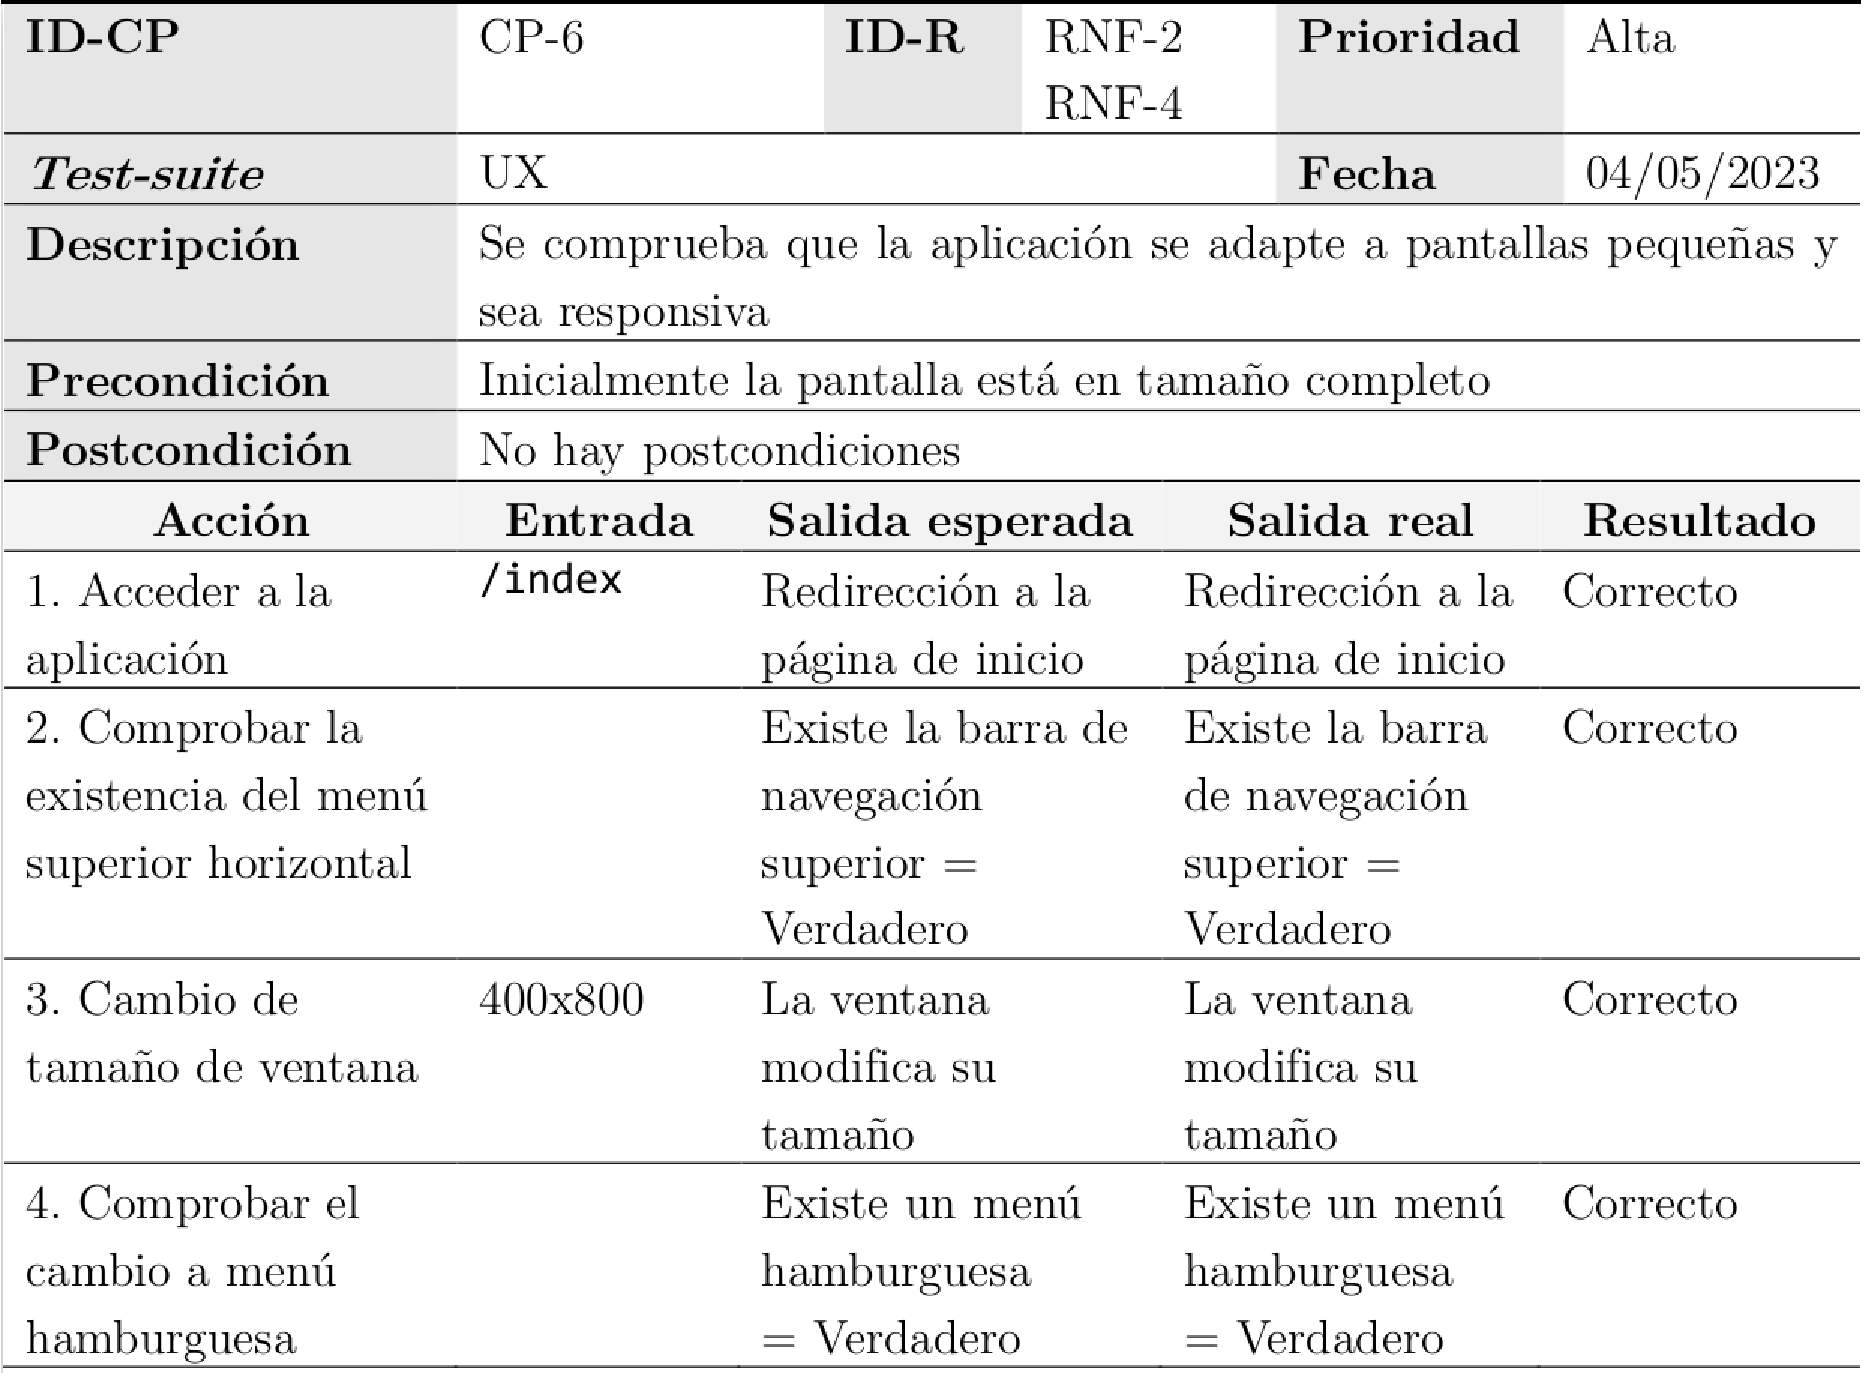
\includegraphics[width=\textwidth]{../img/anexos/cp/CP-6}
	\caption{CP-6 Pantallas responsivas.}
	\label{cp:hamburguer-menu}
\end{table}

\begin{table}[p]
	\centering
	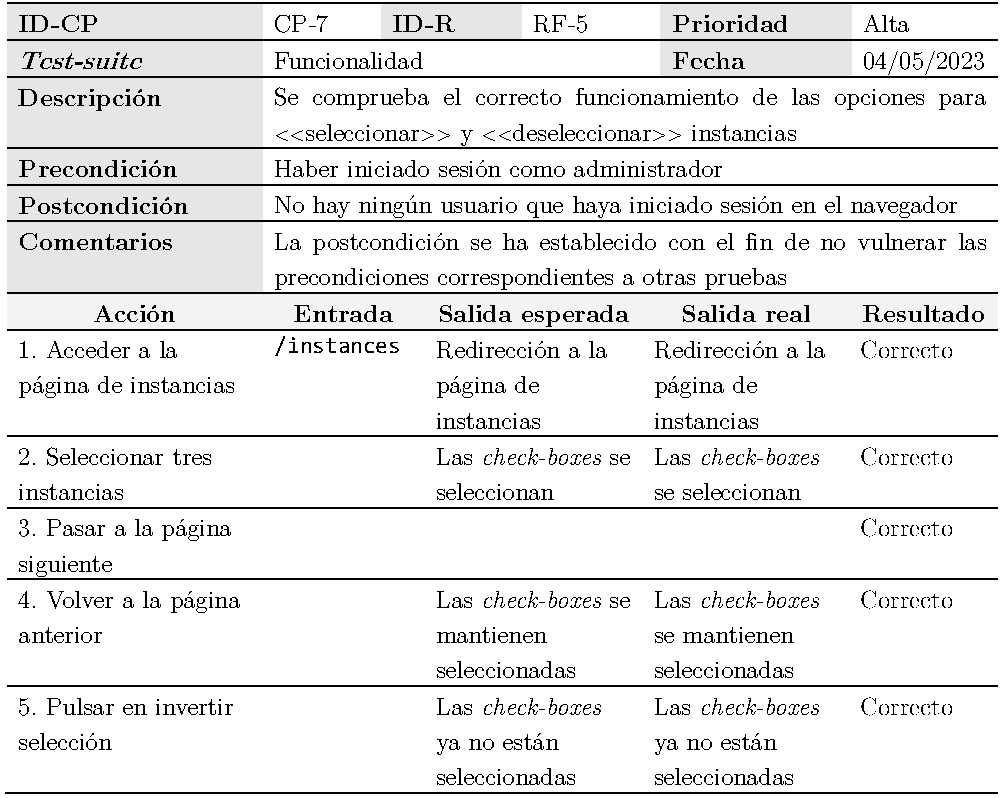
\includegraphics[width=\textwidth]{../img/anexos/cp/CP-7}
	\caption{CP-7 Funcionamiento de las \textit{check-boxes}.}
	\label{cp:checkboxes}
\end{table}

\begin{table}[p]
	\centering
	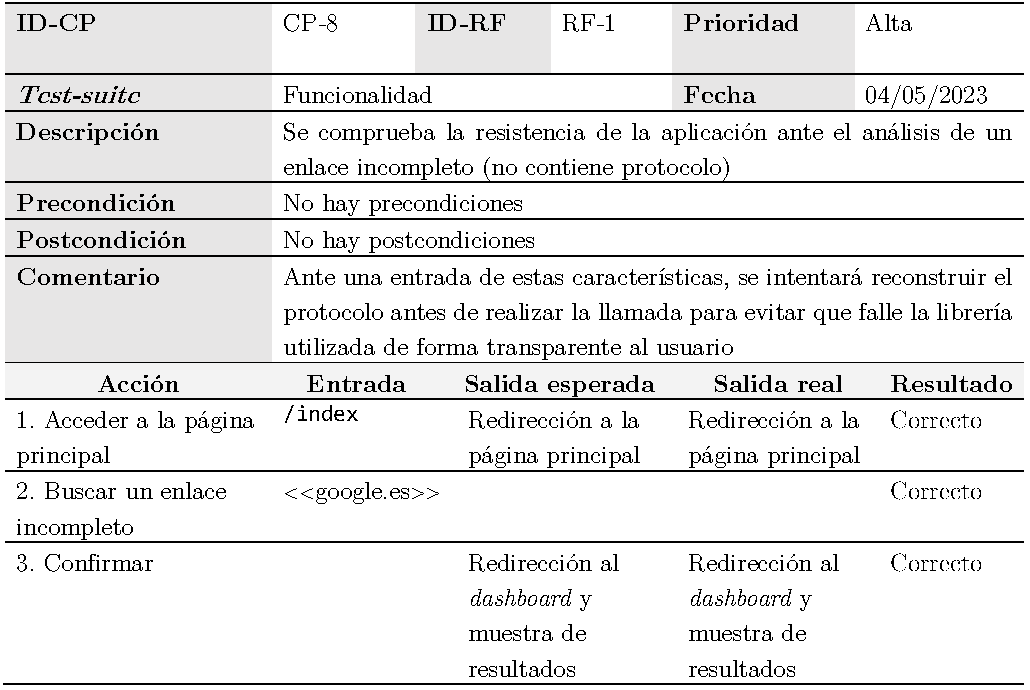
\includegraphics[width=\textwidth]{../img/anexos/cp/CP-8}
	\caption{CP-8 Análisis enlace incompleto.}
	\label{cp:url-incompleta}
\end{table}

\begin{table}[p]
	\centering
	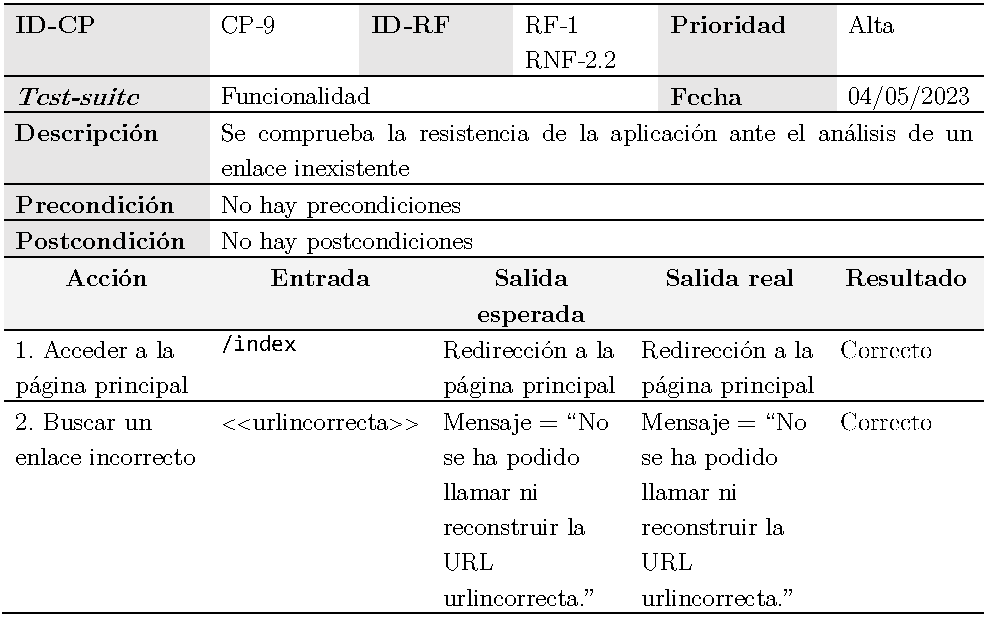
\includegraphics[width=\textwidth]{../img/anexos/cp/CP-9}
	\caption{CP-9 Análisis enlace erróneo.}
	\label{cp:wrong-url}
\end{table}

\begin{table}[p]
	\centering
	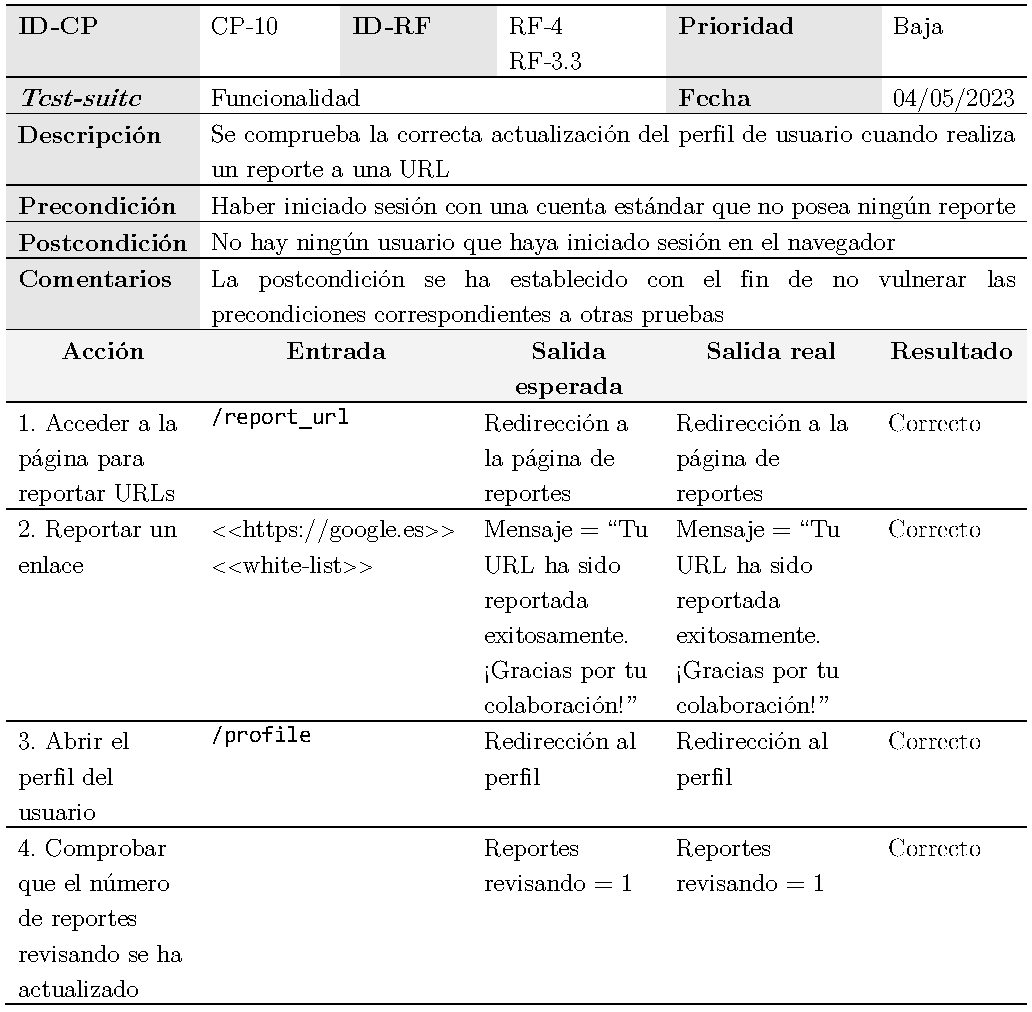
\includegraphics[width=\textwidth]{../img/anexos/cp/CP-10}
	\caption{CP-10 Actualización del perfil con las denuncias de URLs.}
	\label{cp:report-url}
\end{table}

\begin{table}[p]
	\centering
	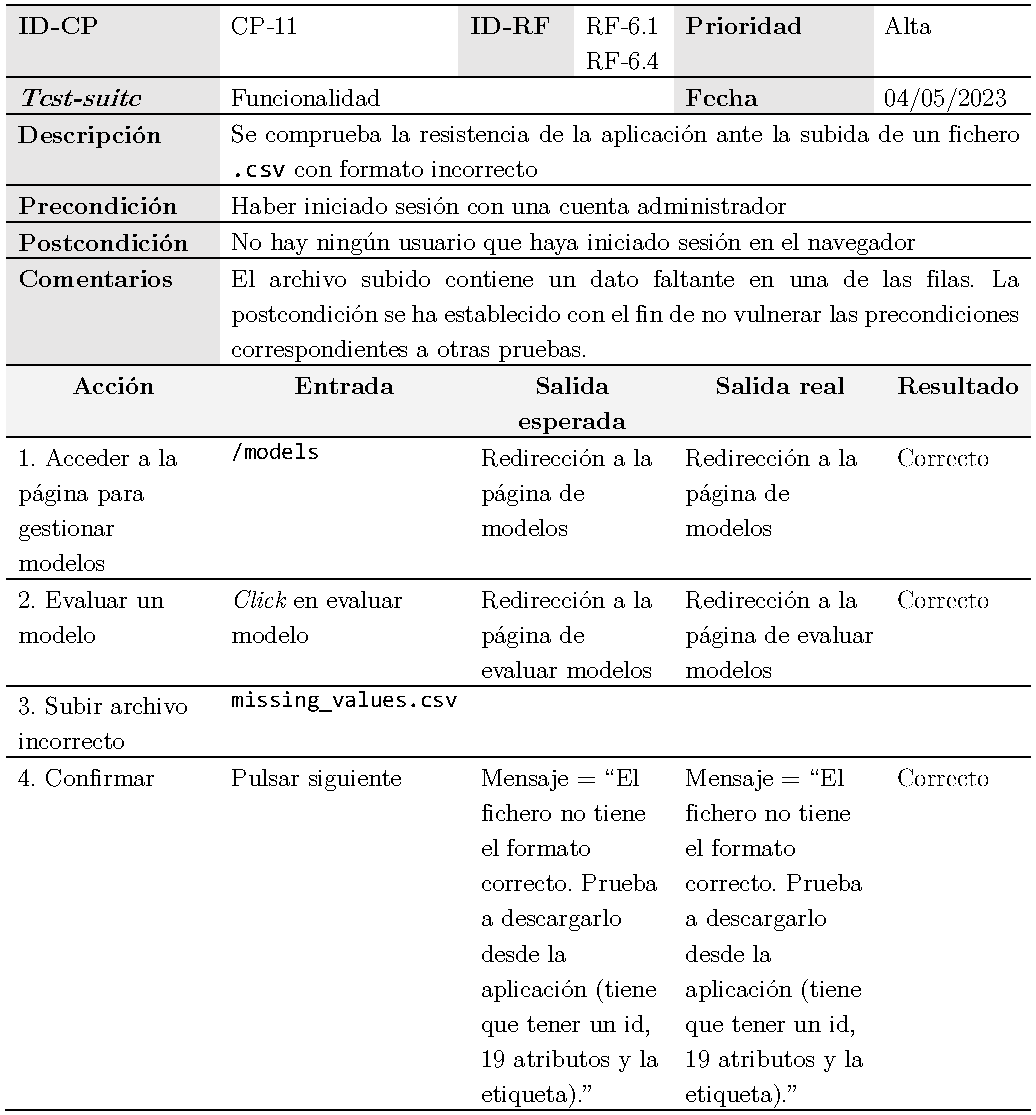
\includegraphics[width=\textwidth]{../img/anexos/cp/CP-11}
	\caption{CP-11 \texttt{csv} con formato incorrecto.}
	\label{cp:wrong-csv}
\end{table}

\begin{table}[p]
	\centering
	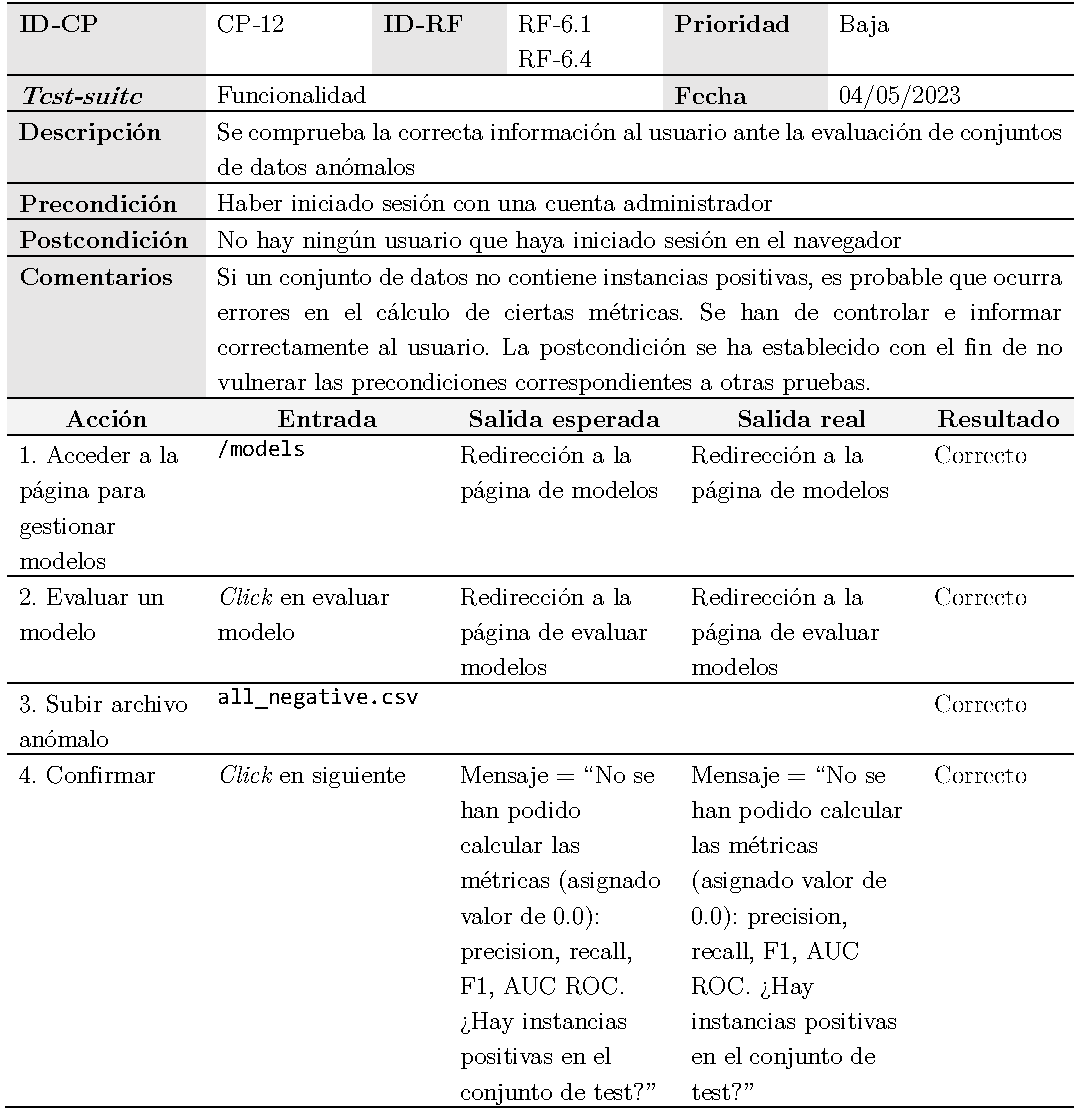
\includegraphics[width=\textwidth]{../img/anexos/cp/CP-12}
	\caption{CP-12 \texttt{csv} con conjunto de \textit{test} anómalo.}
	\label{cp:strange-csv}
\end{table}